\documentclass[twoside,twocolumn]{article}

\usepackage{blindtext} 
\usepackage{graphicx}
\usepackage[sc]{mathpazo} 
\usepackage[T1]{fontenc} 
\linespread{1.05} 
\usepackage{microtype} 


\usepackage[english]{babel} 


\usepackage[hmarginratio=1:1,top=32mm,columnsep=20pt]{geometry} 
\usepackage[hang, small,labelfont=bf,up,textfont=it,up]{caption} 
\usepackage{booktabs} 


\usepackage{lettrine} 


\usepackage{enumitem} 
\setlist[itemize]{noitemsep} 


\usepackage{abstract} 
\renewcommand{\abstractnamefont}{\normalfont\bfseries} 
\renewcommand{\abstracttextfont}{\normalfont\small\itshape} 


\usepackage{titlesec} 
\renewcommand\thesection{\Roman{section}} % 
\renewcommand\thesubsection{\roman{subsection}} 
\titleformat{\section}[block]{\large\scshape\centering}{\thesection.}{1em}{} 
\titleformat{\subsection}[block]{\large}{\thesubsection.}{1em}{} 


\usepackage{fancyhdr} 
\pagestyle{fancy} 
\fancyhead{} 
\fancyfoot{} 
\fancyhead[C]{Inmon vs Kimball $\bullet$ Octubre 2019 $\bullet$ } 
\fancyfoot[RO,LE]{\thepage} 


\usepackage{titling} 


\usepackage{hyperref} 


%----------------------------------------------------------------------------------------
%	TILULOS
%----------------------------------------------------------------------------------------


\setlength{\droptitle}{-4\baselineskip} 

\pretitle{\begin{center}\Huge\bfseries} 
\posttitle{\end{center}} 
\title{Inmon vs Kimball} 
\author{Marko Antonio Rivas Rios\\  Jorge Luis Mamani Maquera
}
\date{\today} 
\renewcommand{\maketitlehookd}{


\noindent 
\begin{center}
Resumen
\end{center}
\textbf{}\\
Este artículo define el almacenamiento de datos y sus conceptos básicos y describe el
punto de vista metodológico entre dos influyentes expertos en almacenamiento de datos Bill Inmon
y Ralph Kimball al proporcionar los mismos atributos, contradicciones, factores influyentes
favoreciendo el enfoque de Inmon y Kimball con un par de proyectos ejecutados en tiempo real
siguiendo algunas de las pautas para determinar el mejor enfoque basado en la referencia
documentos.
\textbf{}\\

\noindent 
\begin{center}
Abstract 
\end{center}
\textbf{}\\
This article defines Data warehousing and its basic concepts and describes the
methodological standpoint between two influential data warehousing experts Bill Inmon
and Ralph Kimball by providing the identical attributes, contradictions, influential factors
favoring Inmon and Kimball approach with a couple of real-time executed projects
following some of the guidelines to determine the best approach based on the referenced
papers.

}

%----------------------------------------------------------------------------------------

\begin{document}

% Print the title
\maketitle

%----------------------------------------------------------------------------------------
%	INTRODUCCION
%----------------------------------------------------------------------------------------

\section{Introduccion}
\lettrine[nindent=0em,lines=3]{A}Estamos viviendo en la era de una revolución de datos, y más corporaciones se están dando cuenta de que para liderar, o en algunos casos, para sobrevivir, necesitan aprovechar su riqueza de datos de manera efectiva.
El almacén de datos, debido a su propuesta única como el repositorio empresarial integrado de datos, está jugando un papel aún más importante en esta situación. Actualmente se practican dos estilos de arquitectura prominentes para construir un almacén de datos: la arquitectura Inmon y la arquitectura Kimball.
Este artículo intenta comparar y contrastar los pros y los contras de cada estilo de arquitectura y recomendar qué estilo seguir basándose en ciertos factores.\textbf{}\\
\textbf{}\\
\textbf{}\\
\textbf{}\\
\textbf{Definición de Inmon: }\\
"Un almacén de datos es una variante de tiempo orientada a temas, integrada y
recopilación no volátil de datos en apoyo del proceso de toma de decisiones de la administración ".
\textbf{}\\
\textbf{Almacén de datos de Inmon: }\\
un repositorio centralizado de una empresa que abarca todas las líneas
de negocios y áreas temáticas que contienen datos integrados de fuentes dispares.
(Inmon 2005)
\textbf{}\\
\textbf{}\\
\textbf{Definición de Kimball:}\\
 "Un almacén de datos es una copia de los datos de la transacción específicamente
estructurado para consulta y análisis ". (Kimball y Ross 2002)\textbf{}\\
\textbf{Data Mart de Kimball: }\\
un tema específico orientado o perteneciente a una línea de negocio individual
que se construyen utilizando modelado dimensional. (Abramson 2004)



%----------------------------------------------------------------------------------------
%	Objetivos
%----------------------------------------------------------------------------------------


\section{Objetivos}

\begin{itemize}
\item 

\textbf{Inmon y Kimball}
\\
\item Comprender las Versiones de Bill Inmon y Ralph Kimball

\item Comprender los pasos de Bill Inmon y Ralph Kimball
\\



\end{itemize}


%----------------------------------------------------------------------------------------
%	Marco teorico
%----------------------------------------------------------------------------------------


\section{Marco teorico}
\begin{enumerate}
\item \textbf{Metodología Inmon}:
Bill Inmon define el almacén de datos como un repositorio centralizado y aboga por un top-down
enfoque de desarrollo que adapta las herramientas de bases de datos relacionales (Extract Transform Load - ETL)
a las necesidades de desarrollo de un almacén de datos de toda la empresa que extrae datos de
varias fuentes y almacenes en datos 'atómicos' con el nivel más bajo de detalle que pasa a través de
área de preparación o aterrizaje. Los marts de datos se crean solo después de que el almacén de datos completo tiene
ha sido creado Por lo tanto, el almacén de datos está en el centro de la Fábrica de información corporativa (CIF),
que proporciona un marco lógico para entregar inteligencia de negocios. (Breslin 2004)\\
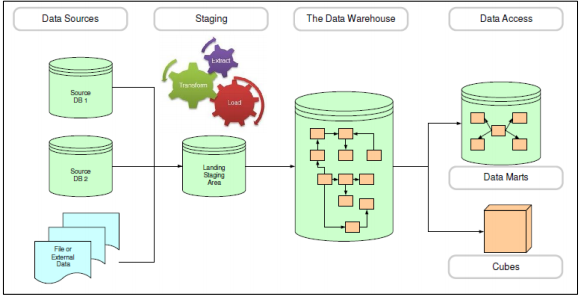
\includegraphics[width=6.5cm]{Imagenes/inmom1}
\\

Inmon divide el entorno general de la base de datos de la organización en cuatro niveles:
\\
1. Operacional
\\
2. Almacén de datos atómicos
\\
3. Departamental
\\
4. Individual

Los últimos tres niveles comprenden el almacén de datos. El primer nivel contiene datos del legado.
y otros sistemas de procesamiento de transacciones. Este nivel es compatible con la operación diaria de
la organización; en otras palabras, el primer nivel admite todo el procesamiento de transacciones. De
En los sistemas operativos, los datos son ampliamente manipulados y luego trasladados a los datos atómicos.
almacén. (Inmon 2005)

\textbf{}
\textbf{El Enfoque de Inmon}\\

El enfoque de Inmon para construir un almacén de datos comienza con el modelo de datos corporativos. Este modelo identifica las áreas temáticas clave y, lo que es más importante, las entidades clave con las que opera y se preocupa la empresa, como el cliente, el producto, el proveedor, etc. A partir de este modelo, se crea un modelo lógico detallado para cada entidad principal. Por ejemplo, se creará un modelo lógico para el Cliente con todos los detalles relacionados con esa entidad. Podría haber diez entidades diferentes bajo Cliente. Todos los detalles, incluidas las claves comerciales, los atributos, las dependencias, la participación y las relaciones, se capturarán en el modelo lógico detallado. El punto clave aquí es que la estructura de la entidad está construida en forma normalizada. La redundancia de datos se evita tanto como sea posible. Esto conduce a una identificación clara de los conceptos comerciales y evita anomalías en la actualización de datos. El siguiente paso es construir el modelo físico. La implementación física del almacén de datos también está normalizada. Esto es lo que Inmon llama como un 'almacén de datos', y aquí es donde se gestiona la versión única de la verdad para la empresa. Este modelo normalizado hace que cargar los datos sea menos complejo, pero usar esta estructura para realizar consultas es difícil ya que involucra muchas tablas y uniones. Entonces, Inmon sugiere construir data marts específicos para los departamentos. Los mercados de datos se diseñarán específicamente para Finanzas, Ventas, etc., y los mercados de datos pueden tener datos desnormalizados para ayudar con los informes (Breslin, 2004). Todos los datos que ingresan al almacén de datos están integrados, y el almacén de datos es la única fuente de datos para los diferentes mercados de datos. Esto garantiza que la integridad y la consistencia de los datos se mantengan intactos en toda la organización.

\textbf{}\\
\textbf{Las ventajas clave del enfoque de Inmon son:}
\textbf{}\\

- El almacén de datos realmente sirve como la única fuente de verdad para la empresa, ya que es la única fuente para los mercados de datos y todos los datos en el almacén de datos están integrados.\textbf{}\\
- Se evitan las anomalías en la actualización de datos debido a la baja redundancia. Esto hace que el proceso ETL sea más fácil y menos propenso a fallas.\textbf{}\\
- Los procesos comerciales se pueden entender fácilmente, ya que el modelo lógico representa las entidades comerciales detalladas.\textbf{}\\
- Muy flexible: a medida que cambian los requisitos comerciales o cambian los datos de origen, es fácil actualizar el almacén de datos, ya que una cosa está en un solo lugar.\textbf{}\\
- Puede manejar diversas necesidades de informes en toda la empresa.\textbf{}\\
\textbf{}\\
\textbf{Estas son algunas de las desventajas del método Inmon:}
\textbf{}\\

- El modelo y la implementación pueden volverse complejos con el tiempo, ya que implica más tablas y combinaciones.\textbf{}\\
- Necesita recursos expertos en modelado de datos y en el negocio mismo. Este tipo de recursos puede ser difícil de encontrar y a menudo son caros.\textbf{}\\
- La configuración inicial y la entrega tomarán más tiempo, y la gerencia debe ser consciente de esto.\textbf{}\\
- Se necesita más trabajo ETL ya que los data marts se crean desde el almacén de datos.\textbf{}\\
- Se necesita un equipo bastante grande de especialistas para administrar con éxito el medio ambiente (Breslin, 2004).\textbf{}\\

\textbf{}\\
\item \textbf{Metodologia Kimboll}: se utiliza para la construcción de un almacén de datos (data warehouse, DW) es decir, una colección de datos situada en un determinado lugar, (empresa, organización, etc.), integrado y variable en el tiempo, ayudando a la toma de decisiones. (Inestroza, 2018) \\

\textbf{Enfoque Kimball}
\\ \\
Contiene varios principios básicos que se analizan detenidamente en el libro de herramientas de Data Warehouse Lifecycle, Second Edition (Kimball, Ross, Mundy, y Becker, 2008)
\begin{itemize}
\item Seguir una metodología comprobada como el  ciclo de vida Kimball.
\item Comprender los requisitos comerciales para priorizar esfuerzos y generar valor comercial. 
\item Diseñar los conjuntos de datos con las características de usabilidad, flexibilidad y rendimiento.
\item Crear y entregar con rapidez los incrementos de los datos basados en procesos comerciales, conocidos con el nombre de almacenamiento de datos. 
\item Diseñar y construir una arquitectura de sistema DW/BI basado en lo que el negocio necesite, según su volumen de datos y entorno de sistemas de TI. 
\item Desarrollar el sistema de extracción, transformación y carga (ETL) con componentes estándar que se encuentran en el entorno de datos analíticos para tratar los patrones de diseño comunes.
\item Brindar la información total, tales como: informes, herramientas de consulta, aplicaciones, portales, documentación, capacitación y soporte.
\end{itemize}



\textbf{Business dimensional lifecycle}
\\ \\
La metodología se basa en lo que Kimball denomina, traducida al español “Ciclo de Vida Dimensional del Negocio”. Basado en cuatro principios básicos:

\begin{itemize}
\item Centrarse en el negocio.
\item Construir una infraestructura de información adecuada.
\item Realizar entregas en incrementos significativos (este principio consiste en crear el almacén de datos (DW) en incrementos entregables en plazos de 6 a 12 meses, en este punto, la metodología se parece a las metodologías ágiles de construcción de software).
\item Ofrecer la solución completa (En este se punto proporcionan todos los elementos necesarios para entregar valor a los usuarios de negocios, para esto ya se debe tener un almacén de datos bien diseñado, se deberán entregar herramientas de consulta ad hoc, aplicaciones para informes y análisis avanzado, capacitación, soporte, sitio web y documentación).

\end{itemize}
La construcción de una solución de DW/BI (Datawarehouse/Business Intelligence) es sumamente compleja, y Kimball plantea una metodología que simplifica esa complejidad. \\ \\
El enfoque del ciclo de vida Kimball se ilustra en el siguiente diagrama. Facilita una hoja de ruta general que constituye la serie de tareas de alto nivel solicitadas para proyectos exitosos de DW / BI.


\includegraphics[width=7.5cm]{Imagenes/Kimboll2}

\textit{"Independientemente de los objetivos específicos de DW / BI de su organización, creemos que un objetivo global del equipo debería ser la aceptación comercial de los entregables de DW / BI para respaldar la toma de decisiones de la empresa. Este objetivo debe permanecer a la vanguardia en todo el diseño, desarrollo e implementación de su sistema DW / BI "} (Arias, 2018)
\\ \\


\textbf{Definicion de requerimientos}

Entre las tareas para definir los requerimientos, existe una flecha bidireccional, esta indica que los requerimientos del negocio son el soporte inicial y también tiene influencia en el plan del proyecto.\\

Si nos fijamos en el centro del diagrama, vemos las tareas asociadas al área de “Datos”, en esta, se diseña e implementa el modelo dimensional, se desarrolla el sub-sistema de extracción, transformación, carga (extract, transformation, and Load-ETL) \\

Las tareas pertenecientes a esta área son:

\begin{itemize}
\item [1.] Modelado Dimensional
\begin{itemize}
\item [1.1.] Elección del proceso de negocio
\item [1.2.] Establecer el nivel de granularidad
\item [1.3.] Elegir las dimensiones
\item [1.4.] Identificar medidas y las tablas de hechos
\end{itemize}
\item [2.] Diseño Físico
\item [3.] Diseño e Implementación del subsistema de Extracción, Transformación y Carga (ETL)
\item [4.] Implementación
\item [5.] Mantenimiento y Crecimiento del Data Warehouse
\textbf{}\\
\textbf{}\\
\item \textbf{Inmon vs Kimball}: \\

Si recordamos lo expuesto en entradas anteriores, el datawarehouse de Kimball está orientado a la consulta de la información, por lo que su estructura interna está especialmente diseñada para garantizar una explotación de los datos rápida y sencilla, no requiriendo usuarios especializados para ello. Por el contrario, el datawarehouse de Inmon persigue la integración de todos los datos de la compañía, estando orientado hacia el almacenaje de grandes volúmenes de datos, por lo que su estructura interna normalizada se diseña para evitar la redundancia de datos, simplificar las labores de mantenimiento, etc. cuestiones que complican las consultas de la información, requiriendo que los usuarios finales estén mucho más especializados. \\
Así, podríamos decir que el enfoque de Kimball se ajusta más a proyectos pequeños en los que se persiga un sistema fácilmente explotable y entendible por el usuario y de rápido desarrollo, siendo el modelo de Inmon más apropiado para sistemas complejos de mayor envergadura. \\
Todo proyecto tiene sus propias peculiaridades, siendo cada caso único e independiente, por lo que resulta necesario llevar a cabo un estudio de todas ellas antes de decantarnos por una solución u otra, de forma que podamos hacernos una idea sobre qué modelo se ajusta mejor a las condiciones de nuestro proyecto. \\
Aun así, tampoco debemos cerrarnos a estas dos opciones, ya que existen casos en los que se han implantado soluciones intermedias entre ambas visiones, logrando así sistemas híbridos que permiten conjugar con éxito las ventajas de ambas perspectivas. \\

\end{itemize}


	
\end{enumerate}





%----------------------------------------------------------------------------------------
%	Ejemplo
%----------------------------------------------------------------------------------------


%----------------------------------------------------------------------------------------
%	Análisis
%----------------------------------------------------------------------------------------





%----------------------------------------------------------------------------------------
%	CONCLUSIONES
%----------------------------------------------------------------------------------------

\section{Conclusiones}
\begin{itemize}	
\item
Se ha demostrado que tanto el enfoque de Inmon como el de Kimball funcionan para entregar con éxito almacenes de datos. Incluso hay organizaciones donde se ha implementado una combinación de ambos ('modelo híbrido'). En un modelo híbrido, el almacén de datos se construye utilizando el modelo Inmon, y además del almacén de datos integrado, los almacenes de datos orientados a procesos de negocio se construyen utilizando el esquema en estrella para la presentación de informes. No podemos generalizar y decir que un enfoque es mejor que el otro; Ambos tienen sus ventajas y desventajas, y ambos funcionan bien en diferentes escenarios. El arquitecto tiene que seleccionar un enfoque para el almacén de datos en función de los diferentes factores; Se identificaron algunas claves en este documento. Finalmente, para que cualquier enfoque sea exitoso, debe ser cuidadosamente pensado, discutido en detalle.
\end{itemize} 



%----------------------------------------------------------------------------------------
%	BIBLIOGRAFIA
%----------------------------------------------------------------------------------------


\begin{thebibliography}{99} 

\bibitem[1]{}
\newblock Arias, D. (4 de marzo de 2018). Todo Sobre La Metodologia Kimball. Obtenido de postparaprogramadores: https://postparaprogramadores.com/metodologia-kimball

\bibitem[2]{}
\newblock Inestroza, M. (18 de Junio de 2018). METODOLOGÍA KIMBALL. Obtenido de goconsultores.com: http://www.goconsultores.com/tag/metodologia-kimball/

\bibitem[3]{}
\newblock Kimball, R., Ross, M., Mundy, J., \& Becker, B. (2008). The Data Warehouse Lifecycle Toolkit, 2nd Edition. Wiley.

\bibitem[4]{}
\newblock Inmon, WH  Construyendo el Data Warehouse, cuarta edición . John Wiley \& Sons., 2005.
\bibitem[5]{}
\newblock Marakas, George M.  Almacenamiento moderno de datos, minería y visualización . Prentice Hall, 2003.
\bibitem[6]{}
\newblock Kimball, Ralph y Margy Ross. The Data Warehouse Toolkit: The Definitive Guide to Dimensional Modeling, Third Edition . John Wiley \& Sons. 2013. Libros 24x7.
\bibitem[7]{}
\newblock Zentut 2016. "Arquitectura del almacén de datos Ralph Kimball" Zentut . com . Consultado el 25 de mayo de 2016. 
\bibitem[8]{}
\newblock Inmon, WH 2010. “UNA CUENTA DE DOS ARQUITECTURAS”
\bibitem[9]{}
\newblock Stanford 2003. "Conceptos de almacenamiento de datos" Stanford.edu. Consultado el 26 de mayo de 2016.

\end{thebibliography}


%----------------------------------------------------------------------------------------


\end{document}
